\section{Baseline concepts}
\label{sec:Baseline}

\subsection{Qubit}
\label{subsec:qubit}

A quantum bit, or \emph{qubit}, is the fundamental unit of quantum information. Physically, it is a quantum-mechanical two-level system, which can be realized in a variety of ways. For example, as the spin of an electron or nucleus that can occupy either a spin-up or spin-down state, or the polarization of a photon that can be horizontal or vertical.

Unlike its classical counterpart, the bit, which can only assume one of the two states 0 or 1, a qubit may exist in a coherent superposition of both basis states. Because of this, the outcome of a measurement is inherently probabilistic, with probabilities determined by the state's probability amplitudes. This ability to exploit superposition, together with other uniquely quantum phenomena such as interference and entanglement, enables quantum algorithms that can outperform their classical counterparts for specific computational problems.

The state of a qubit can be represented in several equivalent ways. One is as a linear combination of the orthonormal computational basis states \(|0\rangle\) and \(|1\rangle\), where the complex amplitudes satisfy the normalization condition \(|\alpha|^2+|\beta|^2=1\)

\begin{equation}
    |\psi\rangle=\alpha|0\rangle+\beta|1\rangle.
    \label{eq:qubitlinearcomb}
\end{equation}

Alternatively, any single-qubit state can be represented geometrically on the \textbf{Bloch sphere}, by a state vector \(\vec{r}\). For a pure state, the state vector has a norm of one and can be parameterized by two angles, \(\theta\) and \(\phi\), as shown in Figure~\ref{fig:blochsphere}. The state vector can be expressed in terms of these angles as

\begin{equation}
    |\psi\rangle=\cos\frac{\theta}{2}|0\rangle+e^{i\phi}\sin\frac{\theta}{2}|1\rangle.
    \label{eq:blochsphere}
\end{equation}

\begin{figure}[ht]
    \centering
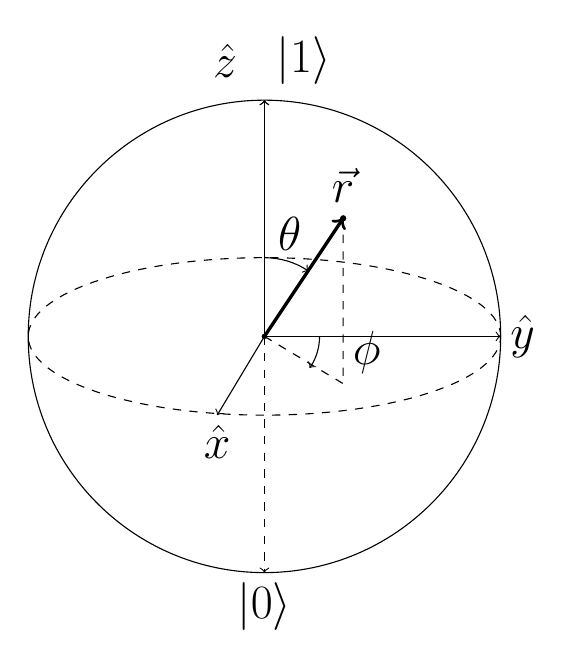
\begin{tikzpicture}[scale=1,font=\LARGE]

  % Radius
  \def\r{3}

  \coordinate (O) at (0,0);
  \coordinate (A) at (\r/3,\r/2);
  \coordinate (P) at (\r/3,-\r/5);

  \draw (O) circle (\r);

  % Equator
  \draw[dashed] (O) ellipse ({\r} and {\r/3});

  \draw[->] (O) -- ++(-\r/5,-\r/3) node[below] {$\hat{x}$};
  \draw[->] (O) -- ++(\r,0) node[right] {$\hat{y}$};
  \draw[->] (O) -- ++(0,\r) node at (-0.5,\r+0.5) {$\hat{z}$};
  \draw[->] (O) -- ++(0,\r) node at (0.5,\r+0.5) {$|1\rangle$};
  \draw[dashed,->] (O) -- ++(0,-\r) node[below] {$|0\rangle$};

  \fill (O) circle (1pt);
  \draw[very thick,->]
    (O) -- (A)
    node[circle,fill,inner sep=0.8pt,label=above:$\vec r$] {};
  \draw[dashed] (O)--(P)--(A);
  
  % Phi
  \draw[->]
    (0.7,0)
    arc[start angle=0,end angle=-35,radius=0.7];
  \node at (1.3,-0.2) {$\phi$};

  % Theta
  \draw[->]
    (0,1.0)
    arc[start angle=90,end angle=56,radius=1.0];
  \node at (0.32,1.3) {$\theta$};

\end{tikzpicture}
    \caption{Representation of a single-qubit state on the Bloch sphere.}
    \label{fig:blochsphere}
\end{figure}


\subsection{Unitary operation}
~\label{subsec:unitary_operation}

A unitary operation is a transformation that is perfectly reversible. For every unitary operation described by a matrix \(U\), there exists an inverse matrix \(U^\dagger\) that describes exactly the undoing of the operation. Consequently, multiplying these two matrices must always equal the identity matrix.

\begin{equation}
    UU^\dagger=U^\dagger U=I
    \label{eq:unitary_identity}
\end{equation}

A unitary operation also preserves the norm of the quantum state vector, and therefore the sum of collapse probabilities. This guarantees that no information is lost throughout the process.

\begin{equation}
    \langle x,y\rangle=\langle Ux,Uy\rangle
    \label{eq:unitary_norm}
\end{equation}

Because of these characteristics, quantum logic gates should aim to implement as close to an unitary operation as possible.

\subsection{Density matrix}
\label{subsec:density_matrix}

\section{The choice of molecule}
\label{sec:choice_of_molecule}

In liquid-state NMR quantum computing, the computational platform consists of an ensemble of molecules containing spin-\(\frac{1}{2}\) nuclei coupled through direct or indirect spin-spin interactions. The molecular structure determines both the number of available qubits and the interactions between them, thereby defining the strategies used for control and quantum information processing.

A key distinction is whether the molecule forms a heteronuclear or homonuclear spin system. In a heteronuclear system, each qubit corresponds to a nucleus of a different chemical species, whereas in a homonuclear system two or more qubits are nuclei of the same species. Since the number of suitable spin-\(\frac{1}{2}\) nuclei is limited, purely heteronuclear systems are generally restricted to a small number of qubits, while larger systems typically contain one or more homonuclear subsystems.

\begin{table}[ht]
    \centering
    \caption{Spin-$\frac{1}{2}$ nuclei commonly used in NMR quantum computing.}
    \label{tab:spin_half_nuclei}

    \begin{tabular}{ccc}
        \toprule
        \textbf{Nucleus} &
        \textbf{Natural abundance (\%)} &
        \makecell[c]{\textbf{Gyromagnetic Ratio} \\
        (\boldmath$\gamma/2\pi$, \textbf{MHz/T})}\\
        \midrule
        $^{1}\mathrm{H}$   & 99.99 & 42.58 \\
        $^{13}\mathrm{C}$  & 1.07  & 10.71 \\
        $^{15}\mathrm{N}$  & 0.37  & $-4.32$ \\
        $^{19}\mathrm{F}$  & 100   & 40.05 \\
        $^{29}\mathrm{Si}$ & 4.68  & $-8.47$ \\
        $^{31}\mathrm{P}$  & 100   & 17.24 \\
        $^{77}\mathrm{Se}$ & 7.63  & 8.13 \\
        \bottomrule
    \end{tabular}
\end{table}

Heteronuclear systems greatly simplify individual qubit addressing because each nucleus possesses a distinct Larmor frequency, allowing selective excitation with radio-frequency pulses. For this reason, they are generally preferred whenever the desired number of qubits permits their use.

\subsection{Dimethyl phosphite}
\label{subsec:dimethyl_phosphite}

The quantum computing platform employed in this work is the heteronuclear molecule dimethyl phosphite, \(\mathrm{{(CH_3O)}_2POH}\), dissolved in a liquid solution within the NMR quantum computer. The two qubits are encoded in the directly bonded \({}^{31}\mathrm{P}\) and \({}^{1}\mathrm{H}\) nuclei located at the center of the molecule, as illustrated in Figure~\ref{fig:dimethyl}.

% Figure: Dimethyl phosphite molecule with qubits highlighted, list of stats of the nuclei

\begin{figure}[ht]
    \centering
\begin{tikzpicture}[scale=1.2]

\pgfdeclarelayer{background}
\pgfsetlayers{background,main}

% Phosphorus
\node[ball color=orange!80,circle,scale=1.4] (P) at (0,0) {$^{31}$P};

% Double-bond oxygen
\node[ball color=red!80,circle,scale=1.2] (O1) at (-1.4,1.4) {O};

% Hydrogen
\node[ball color=white,circle] (H) at (1.4,1.4) {$^{1}$H};

\draw[blue, line width = 2pt] (P) circle (0.70);
\draw[blue, line width = 2pt] (H) circle (0.50);

% Left methoxy
\node[ball color=red!80,circle,scale=1.2] (O2) at (-1.7,-0.9) {O};
\node[ball color=black!70,circle,white,scale=1.2] (C1) at (-3.0,-1.8) {C};

\node[ball color=white,circle] (H11) at (-3.8,-2.4) {H};
\node[ball color=white,circle] (H12) at (-3.5,-0.9) {H};
\node[ball color=white,circle] (H13) at (-2.3,-2.6) {H};

% Right methoxy
\node[ball color=red!80,circle,scale=1.2] (O3) at (1.7,-0.9) {O};
\node[ball color=black!70,circle,white,scale=1.2] (C2) at (3.0,-1.8) {C};

\node[ball color=white,circle] (H21) at (3.8,-2.4) {H};
\node[ball color=white,circle] (H22) at (3.5,-0.9) {H};
\node[ball color=white,circle] (H23) at (2.3,-2.6) {H};

\begin{pgfonlayer}{background}

% Double bond to oxygen
\draw[gray,line width=1mm]
    ($(P)!0.03!(O1)+(0.08,0.08)$) --
    ($(O1)!0.03!(P)+(0.08,0.08)$);

\draw[gray,line width=1mm]
    ($(P)!0.03!(O1)+(-0.08,-0.08)$) --
    ($(O1)!0.03!(P)+(-0.08,-0.08)$);

% P–H bond
\draw[gray,line width=1mm] (P)--(H);

% Single bonds
\draw[gray,line width=1mm] (P)--(H);

\draw[gray,line width=1mm] (P)--(O2);
\draw[gray,line width=1mm] (O2)--(C1);

\draw[gray,line width=1mm] (P)--(O3);
\draw[gray,line width=1mm] (O3)--(C2);

% CH3 groups
\draw[gray,line width=1mm]
(C1)--(H11)
(C1)--(H12)
(C1)--(H13);

\draw[gray,line width=1mm]
(C2)--(H21)
(C2)--(H22)
(C2)--(H23);

\end{pgfonlayer}

\end{tikzpicture}
    \caption{Dimethyl phosphite molecular structure. Nuclei used as qubits are highlighted in blue.}
    \label{fig:dimethyl}
\end{figure}

